% !TEX root = ../journaltemplate.tex

\subsection{Exploring Dust Iron Solubility}

\begin{figure}[h!]
    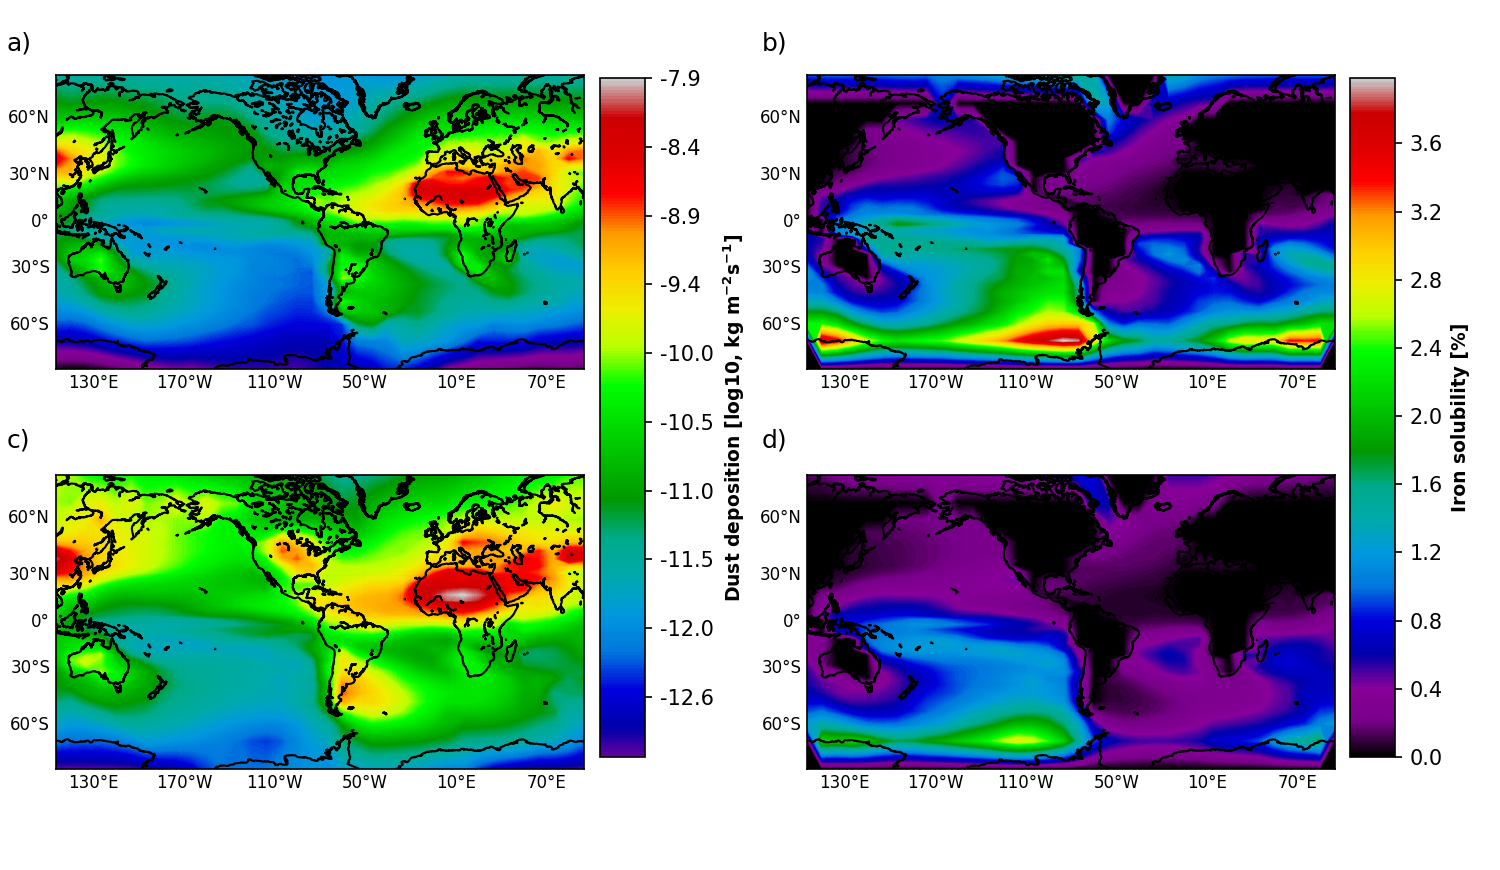
\includegraphics[scale=0.65]{../../Data_function/Function/PicturePaper/Figure7.png}
    \caption{Mean field of (a) Holocene and (c) Last Glacial Maximum (LGM) dust deposition rate derived from the six Holocene-LGM field pairs used in this study, and calculated fractional Fe solubility in deposited dust for the (b) Holocene and (d) LGM.}
\end{figure}


Figure 4 shows the mean fields of dust deposition rate considered in this study for the Holocene (Figure 4a) and LGM (Figure 4c), based on six Holocene-LGM pairs of individual fields as described in section 2.3, as well as the derived mean fields of $\Upsilon_{Fesol}$ in dust aerosols for the Holocene (Figure 4b) and LGM (Figure 4d). The latter constitute the base input fields of soluble Fe for our biogeochemical simulations. 

To properly interpret these results, it is important to clearly identify what processes of Fe solubilization are being captured by our methodology, and which are not. As was mentioned previously, the inverse relationship between $\Upsilon_{Fesol}$ in dust and atmospheric dust load used to derive our $\Upsilon_{Fesol}$ fields is based on laboratory Fe leaching experiments of aerosol samples collected over the ocean using a weakly acidic solution (Baker and Jickells, 2006). Under these conditions, Fe extracted into solution consists of a highly labile Fe fraction that may be extracted in pure water, and a water-insoluble fraction that is solubilized under weakly acidic conditions. Together, these two fractions constitute the so-called labile Fe (Perron et al., 2020). The highly labile fraction of Fe represents non-structural Fe adsorbed onto mineral surfaces, the so-called soluble Fe (Perron et al., 2020), so that leaching experiments performed with pure water (or seawater) mimic Fe solubilization during transport in non-acidic air masses (e.g., Chomchoei et al., 2005; Cosentino et al., 2020; Simonella et al., 2022). This Fe fraction may be considered the source-inherited Fe in dust, readily available without the need of atmospheric processing (Cosentino et al., 2020; Simonella et al., 2020). In turn, the water-insoluble, weak acid-soluble Fe represents structural Fe predominantly in clay minerals (Journet et al., 2008; Marcotte et al., 2020; Simonella et al., 2022), so that Fe leaching experiments with weak acids mimic proton-induced Fe processing during transport in acidic atmospheres (e.g., Cosentino et al., 2020; Simonella et al., 2022). Because soluble Fe is usually a small fraction of labile Fe, as low as 1\% even in close-to-source dust aerosols (e.g., Simonella et al., 2022), and because the relationship we used to derive our input $\Upsilon_{Fesol}$ fields represents labile Fe (Baker and Jickells, 2006), these fields mainly represent Fe solubility enhancement due to progressive fining of dust with greater distance traveled and associated rises in particle reactivity due to higher surface-to-volume ratios (Baker and Jickells, 2006; Cwiertny et al., 2008). Instead, our input fields do not capture differences in source-inherited Fe solubility of dust.


% Please add the following required packages to your document preamble:
% \usepackage{multirow}
\begin{table}[]
    \centering
    \begin{tabular}{||l|l|l|l|l|l|l||}
        \hline 
    \multirow{2}{*}{Model/Region} & \multirow{2}{*}{Global} & \multicolumn{5}{c}{HNLC ocean basin} \\
                                  &                         & NA    & NP    & CEP   & SP    & SAI  \\
    \hline \hline
    MMM\_PI                       & 0.65                    & 0.42  & 0.27  & 0.93  & 1.67  & 1.12 \\
    MMM\_LGM                      & 0.38                    & 0.21  & 0.13  & 0.62  & 1.10  & 0.59 \\
    Albani PI                     & 0.73                    & 0.34  & 0.23  & 0.60  & 1.86  & 1.13 \\
    Albani LGM                    & 0.27                    & 0.18  & 0.09  & 0.63  & 0.53  & 0.28 \\
    Lambert PI                    & 0.36                    & 0.30  & 0.15  & 0.66  & 0.51  & 0.68 \\
    Lambert LGM                   & 0.15                    & 0.12  & 0.06  & 0.35  & 0.20  & 0.44 \\
    Ohgaito PI                    & 0.99                    & 0.49  & 0.29  & 1.18  & 3.68  & 2.04 \\
    Ohgaito LGM                   & 0.35                    & 0.19  & 0.11  & 0.73  & 0.83  & 0.37 \\
    Takemura PI                   & 0.70                    & 0.51  & 0.41  & 0.96  & 1.50  & 1.32 \\
    Takemura LGM                  & 0.65                    & 0.31  & 0.31  & 0.62  & 1.47  & 1.63 \\
    MIROC-ESM PI                  & 0.77                    & 0.44  & 0.30  & 1.04  & 2.39  & 1.40 \\
    MIROC-ESM LGM                 & 0.76                    & 0.22  & 0.14  & 0.60  & 2.67  & 2.06 \\
    MRI-CGCM3 PI                  & 0.58                    & 0.38  & 0.23  & 1.06  & 1.44  & 0.85 \\
    MRI-CGCM3 LGM                 & 0.49                    & 0.29  & 0.16  & 0.89  & 1.44  & 0.70 \\
    \hline
    \end{tabular}
    \caption{Mean fractional iron solubility (\%) in deposited dust aerosols. NA: North Atlantic, NP: North Pacific, CEP: Central East Pacific, SP: South Pacific, SAI: South Atlantic and South Indian, PI: Pre-Industrial, LGM: Last Glacial Maximum. MMM: Multi-Model Mean}
    \end{table}

Table 1 illustrates the average global dust $\Upsilon_{Fesol}$ values for both the Holocene and the Last Glacial Maximum (LGM), alongside regional averages pertaining to the primary High Nutrient Low Chlorophyll (HNLC) ocean basins, considering the different dust fields employed in this study. Due to heightened dust loads during the LGM, dust $\Upsilon_{Fesol}$ reaches a global average of 0.38\%, notably lower than that of the Holocene (0.65\%). While the iron solubility (Fe) during dust transport is recognized to fluctuate up to 10\% with spatial heterogeneity (Journet et al., 2008), several studies adopt a fixed global measurement often below or near 1\% (Lambert et al., 2021; Odalen et al., 2020; Saini et al., 2022; Tagliabue et al., 2016).

The $\Upsilon_{Fesol}$ similarity between Takemura, and MIROC-ESM models is unsurprising, considering that both exclude glaciogenic origin dust source because used a similar aerosol module, while Ohgaito tend to underestimate the glaciogenic dust source originating from latitudes south of 30°S, thereby contributing to greater heterogeneity. The Lambert model displays the most pronounced deviation from the average; nevertheless, it demonstrates the most accurate representation of dust load for both North and South America, encompassing the sources of glaciogenic dust (Lambert et al. 2015).

On a regional scale, the Eastern Central Pacific (CEP), alongside the Southern Oceans (SO), South Pacific (SP), and South Indian Atlantic (SAI), exhibit the most pronounced dissolved iron inputs. Median values of 1.01\% (CEP), 1.71\% (SP), and 0.93\% (SAI) during the Holocene, and 0.62\% (CEP), 1.1\% (SP), and 0.43\% (SAI) during the LGM, respectively, are observed. As all models tend to proficiently replicate conditions in the CEP, it emerges as the region with the most adept concordance between models for both periods.

\subsection{Iron solubility effect on atmospheric carbon dioxide }

\begin{figure}[h!]
    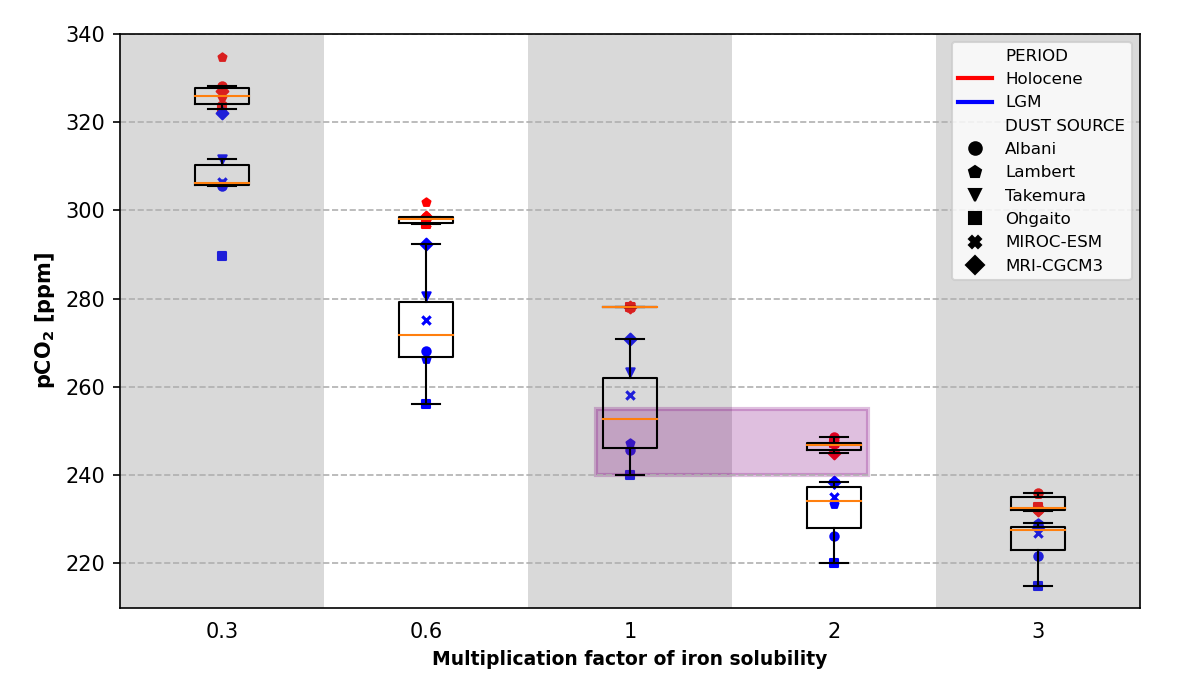
\includegraphics[scale=0.7]{../../Data_function/Function/PicturePaper/Figurex1_Subplot_CO2.png}
    \caption{Partial pressure of atmospheric carbon dioxide (pCO2) concentration for each experiment where iron solubility is multiplied by a factor between 0.3 and 3. Experiments using each of the dust deposition fields for Holocene (in red) and Last Glacial Maximum (LGM, in blue) are shown with different symbols.}
\end{figure} 

\note[N]{expandir caption Figure 4 para explicar los agregados de la figura: valores pCO2 de equilibrio}

As shown in Figure 5, increasing the solubility of Fe results in a decrease in atmospheric CO2 concentration. This relationship exhibits a marked non-linear behavior, suggesting a threshold for efficient Fe utilization, as also observed by Saini et al. (2022).  \annote[Naty]{This effect is also illustrated in Figure xx of the Supplementary Material, which shows that the Holocene and LGM experienced a maximum CO2 decrease of around 91 and 44 ppm, respectively. This finding indicates the point at which atmospheric CO2 concentration would experience no significant change due to the combined influence of dust and Fe solubility.}{Modificar figura original para que no haya suplementaria} 

Control simulations indicate that CO2 sequestration during the Holocene differs from that of the LGM. The variations in CO2 levels during glacial periods are between 7 to 37 ppm lower (Table 3), depending on the type of dust model and the Fe solubility associated with it. When bioavailable Fe levels increase, the difference in atmospheric CO2 between the LGM and Holocene is reduced (Figure 5). These findings suggest a potential buffering effect of Fe in the glacial ocean, which may become saturated more quickly due to the increase in dust flux during this period. 

The significant impact of Fe solubility on atmospheric CO2 capture is demonstrated by the rapid response of marine biomass. Our simulations show that doubling the Fe solubility of the Holocene triggers an average CO2 removal similar to that during the glacial period (see purple box in Figure 5), while tripling it results in a CO2 uptake equivalent to doubling the solubility during the LGM. In other words, doubling the current Fe solubility can lead to a global carbon sequestration comparable to the increase in dust during the last maximum glaciation. Our globally distributed dust fields exhibit LGM:Holocene ratios ranging from 1.4 to 4.7, which are consistent with other studies indicating 2.2 to 6.0 times pre-industrial concentrations (Albani et al., 2016: Lambert et al., 2015; Mahowald et al., 2006; Sudarchikova et al., 2015; Takemura et al., 2009). \annote[Naty]{We also found that at a certain point, when we quadruple the Fe solubility, the CO2 concentrations during both the Holocene and the LGM reach approximately 222 ppm (see Figure xx of the Supplementary Material)}{Sacar lo de figura suplementaria, cambiar por la figura 5}. This suggests that Fe solubility could play a key role in oceanic carbon fixation, which has been overlooked due to the scarcity of paleo-solubility data compared to Fe paleo-flux data. 

\subsection{Regional behavior}

\begin{figure}[h!]
    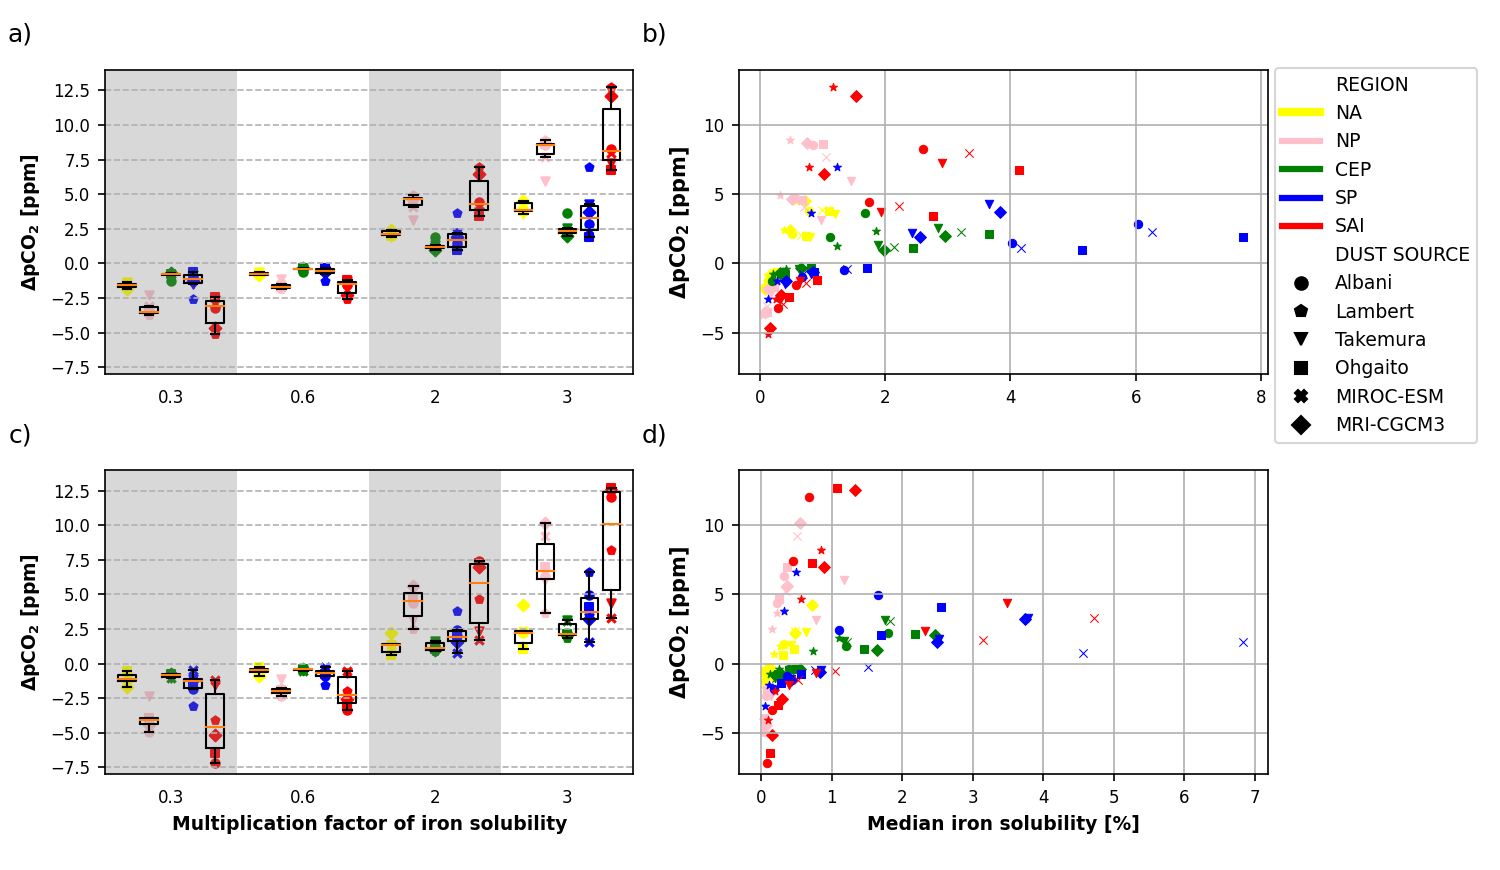
\includegraphics[scale=0.65]{../../Data_function/Function/PicturePaper/Figure4_Final.png}
    \caption{Difference in atmospheric carbon dioxide concentration ($\Delta pCO_2 = pCO_{2,control} - pCO_{2,experiment}$), for each experiment where iron solubility is multiplied by a factor between 0.3 and 3, compared to the same experiment with no factor applied (a and c). Experiments using each of the dust deposition fields for Holocene (a and b) and Last Glacial Maximum (c and d) are shown with different symbols. For each simulation (single data point), the factor of iron solubility was only applied to all grid cells within a specific high-nutrient, low- chlorophyll (HNLC) ocean basin (North Atlantic (NA), North Pacific (NP), Central Eastern Pacific (CEP), South Pacific (SP) and South Atlántic-Indian ocean (SAI)), while iron solubility in all other grid cells in the model was left unchanged. Results are also shown with respect to the median fractional iron solubility of the ocean basin considered (b and d). }
\end{figure}

In terms of regional patterns, our findings align with global trends. Increasing solubility above control levels results in higher CO2 sequestration (Figure 6a, 6c), and conversely. Sensitivity experiments to Fe variation show that during the LGM, CO2 concentration was reduced by 8-11\% above the capture of control simulations. The most significant variations occurred in the South Atlantic-Indian (SAI) region, where the maximum CO2 capture averaged 8.9 ppm. In the Holocene, although the regional patterns replicated those of the LGM, HNLC areas were responsible for a smaller proportion of global CO2 sequestration, accounting for only 44-62\% compared to 61-82\% during the LGM. This difference is likely due to lower dust deposition and a slight reduction in Fe solubility, particularly in HNLC regions relative to glacial periods (Figure 4b and 4d). During this time, the SAI region had an average maximum atmospheric CO2 capture of 9.2 ppm, while the North Atlantic basin became more active. 

Figure 6 illustrates how the Southern Oceans (SO), particularly the SAI basin, exerts a major control over CO2 sequestration, especially during the LGM, despite being highly sensitive to variations in Fe solubility (as shown in Figure 4b and 4d). This increase in sequestration during the LGM could be linked to elevated dust deposition in the region, which was significantly higher during glacial periods, reaching up to 20 times that of the Holocene (as reported by Lamy et al., 2014, and Dome Fuji Ice Core Project members, 2017). However, some models, such as MIROC-ESM and MRI-CGCM3,  tend to underestimate the magnitude of glaciogenic fluxes, possibly due to a lack of agreement in the way each model has been configured to represent vegetation distribution. The North Pacific (NP) basin is the second most active in terms of CO2 capture during both periods. These findings partially align with those of Lambert et al. (2021), with the main difference being observed in the Central-Eastern Pacific (CEP). Although it tends to differ slightly from control simulations in both periods, with maximum differences of 3 ppm for maximum solubility values, the North Atlantic (NA) appears to have the least impact on CO2 reduction during the LGM. Regardless of the Fe solubility value, the simulations show that the capacity to handle bioavailable Fe remains almost unchanged. However, during the Holocene, the CEP basin appears to play a more significant role than the South Pacific (SP) in terms of CO2 sequestration. This trend is possibly associated with weaker Fe deposition in the NA basin relative to the CEP, despite some models reporting increased fluxes from North Africa during the LGM. 

\subsection{Basin efficiency}

\begin{figure}[h!]
    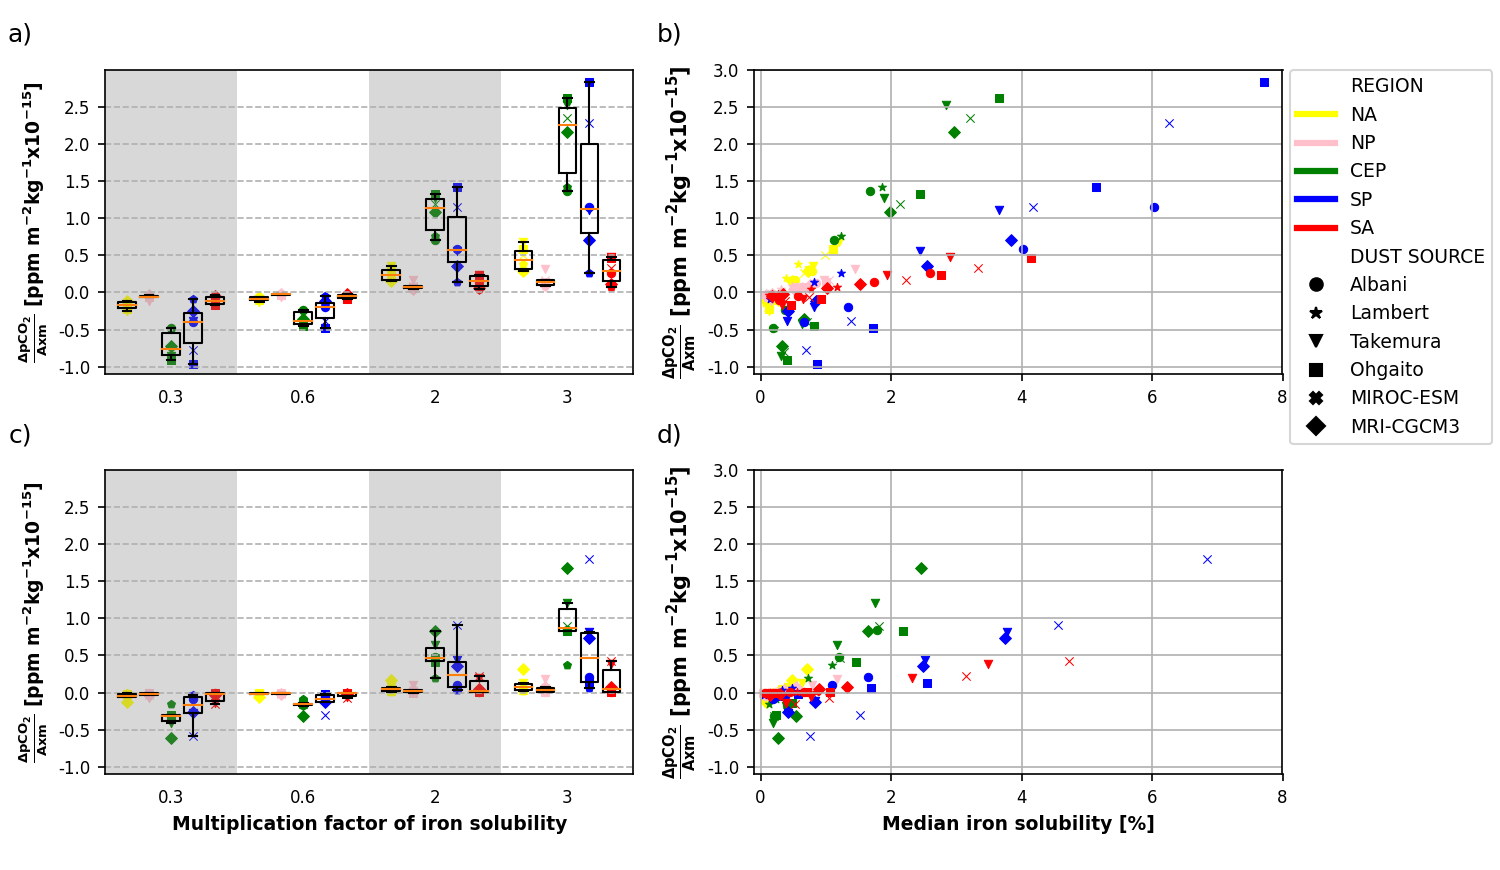
\includegraphics[scale=0.65]{../../Data_function/Function/PicturePaper/Figure6_Subplot_CO2Diff_Normalize.png}
    \caption{Difference in atmospheric carbon dioxide partial pressure (pCO$_2$) as in Figure 6, this time normalized by area and dust deposition load. }
\end{figure}

The contribution of different ocean basins to the total global CO2 reduction due to dust-borne Fe fertilization depends on both the total ocean basin area and the magnitude of iron deposition. When normalizing the CO2 concentration by both factors, it reveals that the SP and CEP basins are the most efficient in using available ocean resources to reduce atmospheric CO2 concentration for both periods (Figure 7). The CEP is an upwelling zone, therefore, a continuous nutrient supply makes this region of vital importance for the biological pump. However, when contrasting the Holocene and the LGM, we can see how the solubility of deposited Fe usually varies between 0.5 and 2.0\%, with lower values during the LGM (Figure 4b and 4d). These values are much lower than those found in the SP basin.  

There are remarkable hemispheric differences between basins (Figure 7b, 7d). While SO seems to display a \annote[N]{gradual}{creo que ac\'a "gradual" est\'a mal usado... discut\'amoslo el lunes} use of bioavailable Fe for CO2 capture, the rest of the HNLC zones show a tendency to be more efficient in utilizing deposited Fe. Therefore, with small amounts, they can achieve the same performance as large basins, as we can see by comparing the behavior of NP and SAI or CEP and SP. While these trends are evident in both periods, the hemispheric differentiation is more notable during the Holocene than during the LGM. The above more prominently demonstrates the saturation effect of Fe under higher rates of dust deposition. 

 